% 第9章第1节：泛函的微分（方向导数、Gâteaux微分、Fréchet微分、Hilbert梯度）。

\section{泛函的微分}
\label{sec:opt-fn-differential}

有限维优化的第一步是看目标在一点附近怎样变化：梯度给出所有方向上的一阶响应。本节对给定函数施加小扰动，建立方向响应、线性近似与梯度三者的关系，暂不加入任何最优性要求。先把候选、目标和定义域说清，因为在函数空间里，目标能否在一点附近取有限值本身就需要检查。

\paragraph{候选空间与目标泛函}
本章的候选$u$是某个实赋范空间$X$中的元素，通常是定义在区间或区域上的函数。从候选到实数（允许取$+\infty$）的映射$J:X\to\mathbb R\cup\{+\infty\}$称为\term{目标泛函}（objective functional），它是一种\term{泛函}（functional）。有效定义域$\operatorname{dom}J=\{u\in X:J(u)<+\infty\}$收集取有限值的候选，可行候选的集合$C\subseteq\operatorname{dom}J$另行记录约束。章首的例子取$X=H^1(0,1)$，目标
\begin{equation}
 J_0(u)=\frac12\int_0^1u'(x)^2\,dx
 \label{eq:opt-fn-dirichlet-energy}
\end{equation}
在整个$H^1(0,1)$上有限；端点条件写进$C=\{u\in H^1(0,1):u(0)=0,\ u(1)=1\}$。这里$u'$是弱导数，端点值取$u$的连续代表在端点处的值：一维$H^1$函数有唯一的连续代表，端点值还受$H^1$范数控制，平方可积函数空间、弱导数与边界值的这些结论见\BookChapterRef{chap:weak-derivatives-sobolev}{卷二“弱导数与Sobolev空间”章}。

\paragraph{目标的来源与定义域}
标量目标可以来自不同的度量。有限个位置上的观测误差$\sum_{i=1}^n(u(x_i)-y_i)^2$要求点值$u\mapsto u(x_i)$在$X$上有意义且连续，这在$H^1(0,1)$中成立，在$L^2(0,1)$的等价类上却没有定义；整体函数值误差$\int_0^1(u-g)^2dx$在$L^2(0,1)$上有限；导数能量~\eqref{eq:opt-fn-dirichlet-energy}要求导数平方可积。三者都给出一个数，但定义域、可微性与约束需要分别核验。讨论微分时，我们总要求$J$在所考察点的某个开邻域内取有限值。例如把$J_0$放到$X=L^2(0,1)$上，令不在$H^1$中的函数取$+\infty$：$L^2$中任意小的球都含有不属于$H^1$的函数，$J_0$在任何一点附近都不全有限，在这个空间里谈不上微分。

\subsection{方向导数}
\label{sec:opt-fn-directional}

固定候选$u$和一个扰动方向$h\in X$，让一个实数$t$控制扰动的大小，候选沿直线$u+th$移动。目标沿这条直线变成一元函数$\varphi(t)=J(u+th)$，我们已经会对它求导。

\begin{definition}[方向导数]
\label{def:opt-fn-directional-derivative}
设$u,h\in X$，且存在$t_0>0$使$|t|<t_0$时$J(u+th)<+\infty$。若极限
\[
 J'(u;h)=\lim_{t\to0}\frac{J(u+th)-J(u)}{t}
\]
存在且有限，则称它为$J$在$u$处沿$h$的\term{方向导数}（directional derivative）。
\end{definition}

定义中的极限是双侧的，所以$J'(u;h)$就是$\varphi'(0)$。由$J(u+t(ch))=J(u+(ct)h)$可知，若$J'(u;h)$存在，则对每个实数$c$有$J'(u;ch)=cJ'(u;h)$；方向导数自动对方向齐次，但定义没有要求它对方向可加。

\paragraph{改变整条曲线，而非输入位置}
取$u(x)=x^2$、$h(x)=\sin(\pi x)$。$h$在两端为零，所以每条$u+th$都满足端点条件。对~\eqref{eq:opt-fn-dirichlet-energy}，$(u+th)'=2x+t\pi\cos(\pi x)$，利用$\int_0^1x\cos(\pi x)\,dx=-2/\pi^2$与$\int_0^1\cos^2(\pi x)\,dx=1/2$，得
\[
 \varphi(t)=J_0(u+th)=\frac23-\frac4\pi t+\frac{\pi^2}4t^2,\qquad J_0'(u;h)=\varphi'(0)=-\frac4\pi\approx-1.273 .
\]
图~\ref{fig:opt-fn-perturbation-family}(a)画出这一族曲线：$t$变化时，整条曲线一起移动，端点不动；(b)中$\varphi$在$t=0$处切线的斜率就是方向导数。它与$u'(x)$是两种不同的导数：$u'(x)$对输入位置$x$求导，衡量一条固定曲线的陡峭程度；$J_0'(u;h)$对标量$t$求导，衡量整条候选曲线变化时目标的响应。(b)中$\varphi$的最小点在$t=8/\pi^3\approx0.258$处，说明沿$h$稍向正方向推动$x^2$可以降低代价，但这只是一条直线上的结论。

\begin{figure}[!htb]
  \centering
  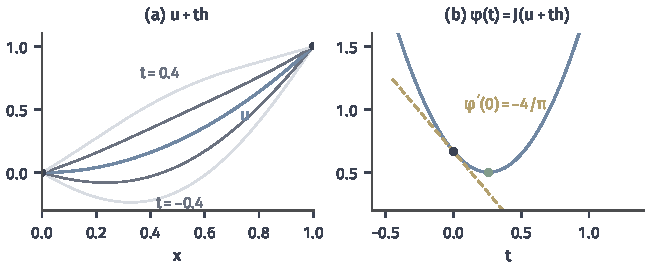
\includegraphics[width=110mm]{figures/03-optimization-evolution-and-signals/01-optimization/matplotlib/c9-perturbation-family/figure.pdf}
  \caption{沿一个方向扰动整条函数。(a)~$u(x)=x^2$（蓝）加上$t\sin(\pi x)$，$t=\pm0.2,\pm0.4$（灰），端点保持在$(0,0)$与$(1,1)$；(b)~目标$J_0(u+th)=\frac23-\frac4\pi t+\frac{\pi^2}4t^2$作为$t$的一元函数，黑点处虚线切线的斜率$-4/\pi$即方向导数，绿点是这条直线上的最小点。}
  \label{fig:opt-fn-perturbation-family}
\end{figure}

\paragraph{参数到函数的映射}
非线性参数拟合中，候选写成$u_{\bm\theta}$，参数$\bm\theta\in\mathbb R^p$的变化先通过映射$\bm\theta\mapsto u_{\bm\theta}$产生函数扰动。沿参数方向$\bm\eta$求导时，候选沿曲线$t\mapsto u_{\bm\theta+t\bm\eta}$而不是直线移动；在下文Fréchet微分的链式法则条件下，参数梯度的第$k$个分量等于目标沿函数方向$\partial u_{\bm\theta}/\partial\theta_k$的响应。参数梯度只看得到这$p$个函数方向，因此它不等于函数空间中的梯度，两者的关系由参数化决定。

\paragraph{各方向都可导，仍不一定线性}
设候选只在二维族$u=a\varphi_1+b\varphi_2$中变化，$\varphi_1,\varphi_2$线性无关，目标经系数写成
\[
 J(a,b)=\frac{a^3}{a^2+b^2}\quad((a,b)\neq(0,0)),\qquad J(0,0)=0 .
\]
在原点沿非零方向$(h_1,h_2)$，$J(th_1,th_2)/t=h_1^3/(h_1^2+h_2^2)$与$t$无关，所以方向导数存在，等于$h_1^3/(h_1^2+h_2^2)$。它对方向不可加：沿$(1,0)$为$1$，沿$(0,1)$为$0$，沿$(1,1)$却是$1/2\neq1+0$。图~\ref{fig:opt-fn-nonlinear-directional}(b)在单位方向$(\cos\theta,\sin\theta)$上画出$\cos^3\theta$；任何线性函数在单位圆上都形如$c_1\cos\theta+c_2\sin\theta$，与$\cos^3\theta$在$\theta=0,\pi/2$处取值相同的只有$\cos\theta$，而两者在$\theta=\pi/4$处已经不同。逐方向求导得到的是一族互不协调的数，还不能像梯度那样统一运算。

\begin{figure}[!htb]
  \centering
  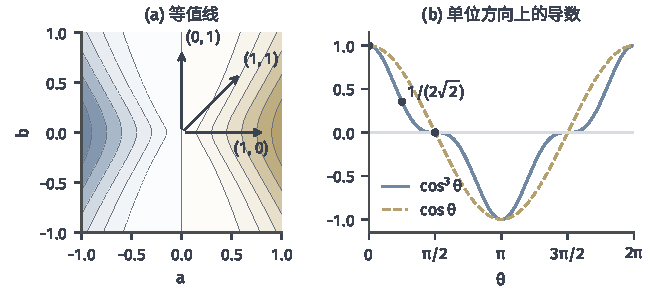
\includegraphics[width=110mm]{figures/03-optimization-evolution-and-signals/01-optimization/matplotlib/c9-nonlinear-directional/figure.pdf}
  \caption{方向导数都存在但不线性的例子$J(a,b)=a^3/(a^2+b^2)$。(a)~$J$的等值线（黄为正、蓝为负）与三个方向$(1,0)$、$(1,1)$、$(0,1)$；(b)~原点处沿单位方向$(\cos\theta,\sin\theta)$的方向导数$\cos^3\theta$（蓝），与线性函数$\cos\theta$（黄虚线）只在少数方向上相同。在$\theta=\pi/4$处前者为$1/(2\sqrt2)$，后者为$1/\sqrt2$。}
  \label{fig:opt-fn-nonlinear-directional}
\end{figure}

\subsection{Gâteaux微分}
\label{sec:opt-fn-gateaux}

上一个例子表明，要把方向响应当成一个对象来运算，还需要它们对方向线性。在函数空间里还要再加一条：响应不能被方向的范数无限放大，否则小扰动可能引起无界的变化。

\begin{definition}[Gâteaux微分]
\label{def:opt-fn-gateaux}
设$J$在$u$的某个开邻域内取有限值。若对每个$h\in X$方向导数$J'(u;h)$都存在，并且映射$h\mapsto J'(u;h)$是$X$上的有界线性泛函，则称$J$在$u$处Gâteaux可微，称这个泛函为$J$在$u$处的\term{Gâteaux微分}（Gâteaux derivative），记作$DJ(u)\in X^*$，$DJ(u)[h]=J'(u;h)$。
\end{definition}

先对每个固定方向取极限，再要求这些极限值组成有界线性泛函，这是本书的约定。有的文献只要求方向导数存在，或只要求线性，就称为Gâteaux可微；阅读时需要核对所用的定义。这里的$X^*$是$X$上全体有界线性泛函构成的对偶空间。

\paragraph{两个基本例子}
设$L:X\to\mathbb R$是有界线性泛函，则$(L(u+th)-Lu)/t=Lh$，所以$DL(u)=L$，与基点$u$无关。再设$X=H$是实Hilbert空间，$J(u)=\|u\|_H^2$。展开内积得
\[
 \frac{\|u+th\|_H^2-\|u\|_H^2}{t}=2\langle u,h\rangle_H+t\|h\|_H^2\longrightarrow2\langle u,h\rangle_H .
\]
映射$h\mapsto2\langle u,h\rangle_H$线性，由Cauchy--Schwarz不等式其范数不超过$2\|u\|_H$，所以$DJ(u)[h]=2\langle u,h\rangle_H$。同样的计算对~\eqref{eq:opt-fn-dirichlet-energy}给出$DJ_0(u)[h]=\int_0^1u'h'\,dx$，它满足$|DJ_0(u)[h]|\le\|u'\|_{L^2}\|h\|_{H^1}$。在这些例子里，方向响应都整理成了对偶空间中的一个元素。

\paragraph{逐方向极限还缺什么}
Gâteaux微分的定义只说：对每个固定的$h$，$t\to0$时误差相对于$t$趋于零。不同方向的趋零速度可以完全不同，定义对此不加控制。当扰动不沿任何固定直线、而是沿一条曲线趋于零时，线性近似可能失效；下一小节先给出这一要求，再用例子说明它确实更强。

\subsection{Fréchet微分}
\label{sec:opt-fn-frechet}

我们希望一个线性对象能同时预测所有足够小的扰动，而不仅是沿每条直线的扰动。这需要把误差相对于扰动的范数统一地控制住。

\begin{definition}[Fréchet微分]
\label{def:opt-fn-frechet}
设$J$在$u$的某个开邻域内取有限值。若存在有界线性泛函$A\in X^*$，使
\begin{equation}
 J(u+h)=J(u)+Ah+r(h),\qquad\lim_{\|h\|_X\to0}\frac{|r(h)|}{\|h\|_X}=0 ,
 \label{eq:opt-fn-frechet}
\end{equation}
则称$J$在$u$处Fréchet可微，$A$称为$J$在$u$处的\term{Fréchet微分}（Fréchet derivative）。余项条件常简写为$r(h)=o(\|h\|_X)$。
\end{definition}

余项条件中的极限对所有趋于零的$h$统一成立，与$h$沿什么路径趋于零无关。由此可以推出Gâteaux可微：固定$h\neq0$，令$t\to0$，则$\|th\|_X\to0$，
\[
 \Bigl|\frac{J(u+th)-J(u)}{t}-Ah\Bigr|=\frac{|r(th)|}{|t|}=\frac{|r(th)|}{\|th\|_X}\|h\|_X\longrightarrow0 .
\]
所以Fréchet可微时$J'(u;h)=Ah$对每个$h$成立，$A=DJ(u)$；两种微分若都存在则相同，以后统一记为$DJ(u)$。Fréchet可微还推出$J$在$u$处连续，因为$|J(u+h)-J(u)|\le\|A\|\|h\|_X+|r(h)|\to0$。

\paragraph{Gâteaux可微而非Fréchet可微}
在$\mathbb R^2$上取
\[
 f(a,b)=\frac{a^3b}{a^4+b^2}\quad((a,b)\neq(0,0)),\qquad f(0,0)=0 .
\]
由$a^4+b^2\ge2a^2|b|$得$|f(a,b)|\le|a|/2$，$f$在原点连续。沿方向$(h_1,h_2)$，$h_2\neq0$时$f(th_1,th_2)/t=t\,h_1^3h_2/(t^2h_1^4+h_2^2)\to0$，$h_2=0$时$f$恒为零，所以所有方向导数都是$0$：$f$在原点Gâteaux可微，微分为零泛函。然而沿抛物线$b=a^2$有$f(a,a^2)=a/2$；当$0<|a|\le1$时$\|(a,a^2)\|_2\le\sqrt2|a|$，余项比$|f(a,a^2)|/\|(a,a^2)\|_2\ge1/(2\sqrt2)$不趋于零，Fréchet条件~\eqref{eq:opt-fn-frechet}不成立。图~\ref{fig:opt-fn-gateaux-not-frechet}(b)显示了原因：沿每条固定射线，比值最终趋于零，但射线越贴近抛物线，开始下降的位置越靠近原点；抛物线从所有射线之间穿过，比值保持在$1/2$附近。

\begin{figure}[!htb]
  \centering
  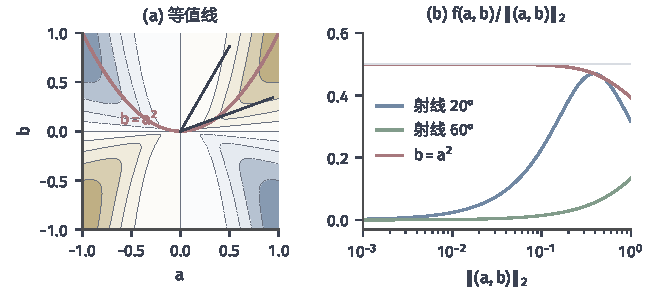
\includegraphics[width=110mm]{figures/03-optimization-evolution-and-signals/01-optimization/matplotlib/c9-gateaux-not-frechet/figure.pdf}
  \caption{Gâteaux可微但非Fréchet可微的$f(a,b)=a^3b/(a^4+b^2)$。(a)~等值线（黄为正、蓝为负）、两条过原点的射线（黑）与抛物线$b=a^2$（红）；(b)~比值$f/\|(a,b)\|_2$随到原点距离的变化（横轴对数）。沿$20^\circ$与$60^\circ$射线比值趋于零，沿抛物线趋于$1/2$。}
  \label{fig:opt-fn-gateaux-not-frechet}
\end{figure}

\paragraph{平方范数与平方误差}
对上一小节的两个例子保留完整的余项。平方范数满足$\|u+h\|_H^2=\|u\|_H^2+2\langle u,h\rangle_H+\|h\|_H^2$，余项$\|h\|_H^2$除以$\|h\|_H$后趋于零，所以它Fréchet可微。设$L\in X^*$，$y\in\mathbb R$，平方误差$E(u)=\frac12(Lu-y)^2$满足
\[
 E(u+h)=E(u)+(Lu-y)\,Lh+\tfrac12(Lh)^2,\qquad\tfrac12(Lh)^2\le\tfrac12\|L\|^2\|h\|_X^2 ,
\]
余项同样是$o(\|h\|_X)$，所以$DE(u)[h]=(Lu-y)Lh$。有限个这样的项相加时，余项相加仍是$o(\|h\|_X)$，这就是和法则；有限观测的平方误差$\frac12\sum_i(L_iu-y_i)^2$的微分是$\sum_i(L_iu-y_i)L_ih$。

\paragraph{链式法则}
复合映射的微分需要把内层映射也纳入同样的框架。设$Y$是赋范空间，映射$T:X\to Y$在$u$处Fréchet可微，指存在有界线性算子$DT(u):X\to Y$使$\|T(u+h)-T(u)-DT(u)h\|_Y=o(\|h\|_X)$。

\begin{theorem}[链式法则]
\label{thm:opt-fn-chain-rule}
设$T:X\to Y$在$u$处Fréchet可微，$G:Y\to\mathbb R\cup\{+\infty\}$在$T(u)$处Fréchet可微。则$G\circ T$在$u$处Fréchet可微，且
\[
 D(G\circ T)(u)[h]=DG(T(u))\bigl[DT(u)h\bigr] .
\]
\end{theorem}

\begin{proof}
记$k(h)=T(u+h)-T(u)$，$s(h)=k(h)-DT(u)h$，则$\|s(h)\|_Y=o(\|h\|_X)$，并且对足够小的$h$有$\|k(h)\|_Y\le(\|DT(u)\|+1)\|h\|_X$，所以$k(h)\to0$，$G$在$T(u+h)$处有限。由$G$的Fréchet可微性，$G(T(u+h))-G(T(u))=DG(T(u))[k(h)]+r_G(k(h))$，其中$r_G(k)=o(\|k\|_Y)$。代入$k(h)=DT(u)h+s(h)$，
\[
 \begin{aligned}
 &G(T(u+h))-G(T(u))-DG(T(u))[DT(u)h]\\
 &\qquad=DG(T(u))[s(h)]+r_G(k(h)) .
 \end{aligned}
\]
第一项的绝对值不超过$\|DG(T(u))\|\,\|s(h)\|_Y$，它是$o(\|h\|_X)$；第二项满足$|r_G(k(h))|\le\varepsilon\|k(h)\|_Y\le\varepsilon(\|DT(u)\|+1)\|h\|_X$，其中$\varepsilon$可随$h\to0$任意小。两项都是$o(\|h\|_X)$。
\end{proof}

最常用的情形是仿射内层映射$T(u)=Bu+b$，其中$B$是有界线性算子，此时$DT(u)=B$，余项$s\equiv0$。

\paragraph{积分目标与范数的选择}
对~\eqref{eq:opt-fn-dirichlet-energy}，$J_0(u+h)-J_0(u)-\int_0^1u'h'\,dx=\frac12\|h'\|_{L^2}^2\le\frac12\|h\|_{H^1}^2$，所以它在$H^1(0,1)$上Fréchet可微。一般的积分目标在把极限移入积分号之前，还要核验支配与可积条件，具体计算留到第~\ref{sec:opt-fn-integral}节。余项是否为$o(\|h\|_X)$取决于所选范数：同一个$J_0$在$L^2$范数下连有限邻域都没有。更换候选空间或范数时，Fréchet可微性必须重新检查。

\subsection{Hilbert梯度}
\label{sec:opt-fn-hilbert-gradient}

微分$DJ(u)$是对偶空间中的元素，它接收方向、返回数值；梯度下降需要的却是候选空间中的一个元素，以便写出$u-\eta\cdot(\text{某个方向})$。在Hilbert空间中，二者可以借内积互相转换。

\paragraph{由微分到梯度}
实Hilbert空间$H$上的每个有界线性泛函$\ell$都有唯一的$g\in H$使$\ell(h)=\langle g,h\rangle_H$对所有$h$成立，并且$\|\ell\|=\|g\|_H$。这就是Riesz表示定理，其证明及对偶空间的一般讨论见\BookChapterRef{chap:linear-functionals-operators}{卷二“线性泛函与线性算子”章}。把它用于$\ell=DJ(u)$，得到
\begin{equation}
 DJ(u)[h]=\langle\nabla_HJ(u),h\rangle_H\qquad\text{对所有}h\in H ,
 \label{eq:opt-fn-hilbert-gradient}
\end{equation}
称$\nabla_HJ(u)\in H$为$J$在$u$处关于内积$\langle\cdot,\cdot\rangle_H$的\term{梯度}（gradient）。由Cauchy--Schwarz不等式，在单位方向$\|h\|_H=1$中，$DJ(u)[h]\ge-\|\nabla_HJ(u)\|_H$，等号在$h=-\nabla_HJ(u)/\|\nabla_HJ(u)\|_H$时取到。下降最快的方向取决于用哪个内积计量“单位方向”。一般Banach空间中没有这样的表示，微分仍留在$X^*$中，不预设一个同空间的梯度。

\paragraph{同一个微分，不同的梯度}
在仿射函数$u(x)=a+bx$构成的二维空间上，固定目标$J(u)=(a^2+b^2)/2$。对方向$h=\alpha+\beta x$，$DJ(u)[h]=a\alpha+b\beta$，这个微分与内积无关。若按系数取内积$\langle u,h\rangle=a\alpha+b\beta$，梯度就是系数$(a,b)$对应的函数$a+bx$。若改用$[-1,1]$上的归一化$L^2$内积$\langle f,g\rangle=\frac12\int_{-1}^1fg\,dx$，则$\langle1,1\rangle=1$、$\langle1,x\rangle=0$、$\langle x,x\rangle=1/3$；寻找$c+dx$使$c\alpha+d\beta/3=a\alpha+b\beta$对所有$\alpha,\beta$成立，得$c=a$、$d=3b$，梯度是$a+3bx$。目标的微分没有改变，改变的只是用哪个元素代表它。若改动目标中观测的权重或能量的权重，改变的才是优化问题本身。

\paragraph{$L^2$梯度与$H^1$梯度}
同样的现象在无限维中有更直观的后果。在$H_0^1(0,1)$上考虑微分$\ell(h)=\int_0^1rh\,dx$，例如它是$J(u)=\frac12\int_0^1(u-g)^2dx$在$u-g=r$处的微分。若用$L^2$内积，梯度就是$r$。若用$H^1$内积$\langle w,h\rangle_{H^1}=\int_0^1(wh+w'h')\,dx$，取$r=\sum_kr_k\sin(k\pi x)$为有限正弦和，令
\[
 w=\sum_k\frac{r_k}{1+k^2\pi^2}\sin(k\pi x) .
\]
$w$光滑、两端为零，并满足$w-w''=r$。对任意$h\in H_0^1(0,1)$分部积分，边界项因$h(0)=h(1)=0$而消失，$\int_0^1(wh+w'h')\,dx=\int_0^1(w-w'')h\,dx=\int_0^1rh\,dx$，所以$w$就是$H^1$梯度。第$k$个频率被除以$1+k^2\pi^2$：图~\ref{fig:opt-fn-l2-h1-gradient}取$r=\sin(\pi x)+0.5\sin(15\pi x)$，高频成分相对低频的比例从$0.5$降到约$0.0024$。用$H^1$梯度作下降步，每一步加到候选上的修正更光滑。离散的梯度型更新沿用第~\ref{chap:opt-smooth}章的算法，连续时间的梯度流留给第~\ref{part:dynamical-systems-control-and-decision}部分。反过来也要注意，$L^2$梯度并不总在候选空间中：$DJ_0(u)[h]=\int u'h'$要写成$\int gh$，需要$u$有平方可积的二阶导数，此时$g=-u''$。

\begin{figure}[!htb]
  \centering
  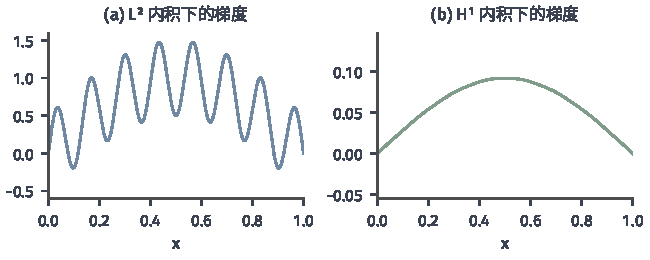
\includegraphics[width=110mm]{figures/03-optimization-evolution-and-signals/01-optimization/matplotlib/c9-l2-h1-gradient/figure.pdf}
  \caption{同一个微分$h\mapsto\int_0^1rh\,dx$在两种内积下的梯度。(a)~$L^2$梯度$r=\sin(\pi x)+0.5\sin(15\pi x)$；(b)~$H_0^1(0,1)$上$H^1$内积下的梯度$w=\sin(\pi x)/(1+\pi^2)+0.5\sin(15\pi x)/(1+225\pi^2)$，高频成分几乎被抹平。两图纵轴尺度不同。}
  \label{fig:opt-fn-l2-h1-gradient}
\end{figure}
